\documentclass[landscape]{article} % kind of document 
\usepackage[utf8]{inputenc} %encoding of choice
\usepackage[american]{babel} %language of choice
\usepackage[p,osf]{cochineal}
\usepackage{fancyhdr} %for header
\usepackage{amsmath, tabu} %math mode
\usepackage{mathtools}
\usepackage{extarrows} % for more options with arrows
\usepackage{amssymb} %math symbols
\usepackage{dsfont} %specifically for the indicator function symbol
\usepackage{xcolor} %to color text
\usepackage{amsthm} %math theorem
\usepackage{tikz}
\usepackage{caption}
\usepackage{multirow}
\usepackage[bottom]{footmisc}
% \usepackage[dvipsnames]{xcolor}
%\usepackage{pythontex}
\usepackage{enumerate} %make lists
\usepackage{graphicx} %insert images
\usepackage{float} %to fix image position
\usepackage{moreverb} %to make boxes
\usepackage{hyperref} %to create hyperlinks
\usepackage{lipsum} %lorem ipsum package
\usepackage{setspace} % to use singlespace below in the solution environment
\usepackage[shortlabels]{enumitem}
\usepackage{parskip}
\usepackage[us]{datetime} %package for setting due date in US format
\newdate{duedate}{6}{12}{2021} %to set a due date
\allowdisplaybreaks
\usepackage[margin=.5in, landscape]{geometry}
\usepackage{rotating}
\usepackage{pdflscape}
\usepackage[paper=portrait,pagesize]{typearea}
\usepackage{jlcode}
\pagestyle{fancy}


\fancypagestyle{mylandscape}{
	\fancyhf{} %Clears the header/footer
	\fancyfoot{% Footer
		\makebox[\textwidth][r]{% Right
			\rlap{\hspace{.75cm}% Push out of margin by \footskip
				\smash{% Remove vertical height
					\raisebox{4.87in}{% Raise vertically
						\rotatebox{90}{\thepage}}}}}}% Rotate counter-clockwise
	\renewcommand{\headrulewidth}{0pt}% No header rule
	\renewcommand{\footrulewidth}{0pt}% No footer rule
}

\lhead{Due: \displaydate{duedate}}
\chead{ECON 899 -- PS3b -- }
\rhead{Danny, Hiroaki, Mitchell, Ryan, Yobin}

\newcommand{\E}[1]{\mathbb{E}\left[#1\right]} %ease of writing e and E
\newcommand{\Ee}[1]{\mathbb{E}_{\epsilon}\left[#1\right]}
\newcommand{\Eep}[1]{\mathbb{E}_{\epsilon'}\left[#1\right]}
\newcommand{\e}{\mathrm{e}}
\newcommand{\ct}{\mathsf{c}}
\newcommand{\Z}{\mathbb{Z}}
\renewcommand{\L}{\mathcal{L}}
\newcommand{\R}{\mathbb{R}}
\newcommand{\N}{\mathbb{N}}
\newcommand{\ifn}{\mathds{1}}
\newcommand{\X}{\mathbf{X}}
\newcommand{\Y}{\mathbf{Y}}
\newcommand{\one}[1]{\mathbf{1}\left\{#1\right\}}
\newcommand{\usmax}[1]{\underset{#1}{\text{max }}}
\newcommand{\loge}[1]{\text{log}\left(#1\right)}
\newcommand\numberthis{\addtocounter{equation}{1}\tag{\theequation}}
\newcommand*\widebar[1]{\overline{#1}} % to get a widebar
\theoremstyle{definition}
\newtheorem{theorem}{theorem} % Theorem display format
\newtheorem{problem}[theorem]{Exercise} % Problem display format, last bracket sets display choice

\newenvironment{solution}[1][Answer]{\begin{singlespace}\underline{\textbf{#1:}}\quad }{\ \rule{0.3em}{0.3em}\end{singlespace}} % Answer format

\newenvironment{solutions}[1][Proof]{\begin{singlespace}\underline{\textbf{#1:}}\quad }{\ \rule{0.3em}{0.3em}\end{singlespace}} % Answer format
\title{Econ899 PS1b}
\usepackage{listings}

\begin{document}
%\maketitle
The code used to complete this problem set is attached in the appendix below. \bigskip \\
The expected value function can be written as:\begin{align*}
	\Ee{V(i, c, p, \epsilon)} &= \Ee{\usmax{a\in\{0, 1\}} U(a|i,c,p,\epsilon) + \beta\sum_{c',p'}\Eep{V(i',c',p',\epsilon')}\Pr(c',p'|c,p,a)} \\
	\Ee{V(s, \epsilon)} &= \Ee{\usmax{a\in\{0, 1\}} U(a|s,\epsilon) + \beta\sum_{s'}\Eep{V(s', \epsilon')}\Pr(s'|s,a)} \\
	\overline{V}(s) &= \Ee{\usmax{a\in\{0, 1\}} U(a|s,\epsilon) + \beta\sum_{s'}\overline{V}(s')\Pr(s'|s,a)} 
\end{align*}
The numerical value for each state variable, $s$, is in the first column below, with the implied value function from $\hat{P}(s)$ in the second column. As you can see, the expected values are much higher using $\hat{P}(s)$, for each state. \begin{equation}
\left[
\begin{array}{cc}
61.13 & 60.91 \\
65.01 & 64.8 \\
68.48 & 68.27 \\
71.67 & 71.44 \\
74.63 & 74.38 \\
77.39 & 77.1 \\
79.96 & 79.59 \\
82.26 & 81.74 \\
84.07 & 83.38 \\
58.49 & 58.27 \\
63.13 & 62.91 \\
67.01 & 66.8 \\
70.48 & 70.27 \\
73.67 & 73.43 \\
76.63 & 76.38 \\
79.39 & 79.1 \\
81.96 & 81.59 \\
84.26 & 83.64 \\
63.24 & 63.0 \\
66.89 & 66.68 \\
70.2 & 69.98 \\
73.26 & 73.01 \\
76.11 & 75.84 \\
78.77 & 78.44 \\
81.2 & 80.74 \\
83.28 & 82.68 \\
84.28 & 83.31 \\
61.03 & 60.81 \\
65.24 & 65.03 \\
68.89 & 68.68 \\
72.2 & 71.98 \\
75.26 & 75.02 \\
78.11 & 77.84 \\
80.77 & 80.4 \\
83.2 & 82.77 \\
85.28 & 84.68 \\
\end{array}
\right]
\end{equation}

\newpage
The log-likelihood function is \[
	\L(s_i|\lambda) = \sum_ia_i\loge{P(s_i)} + (1-a_i)\loge{1 - P(s_i)}
\]
Solving this log-likelihood function using a nested fixed point algorithm yields a result of $\hat{\lambda}=-4.024$. The negative log-likelihood function is plotted below, displaying a unique minimum between -10 and 0.
\begin{center}
	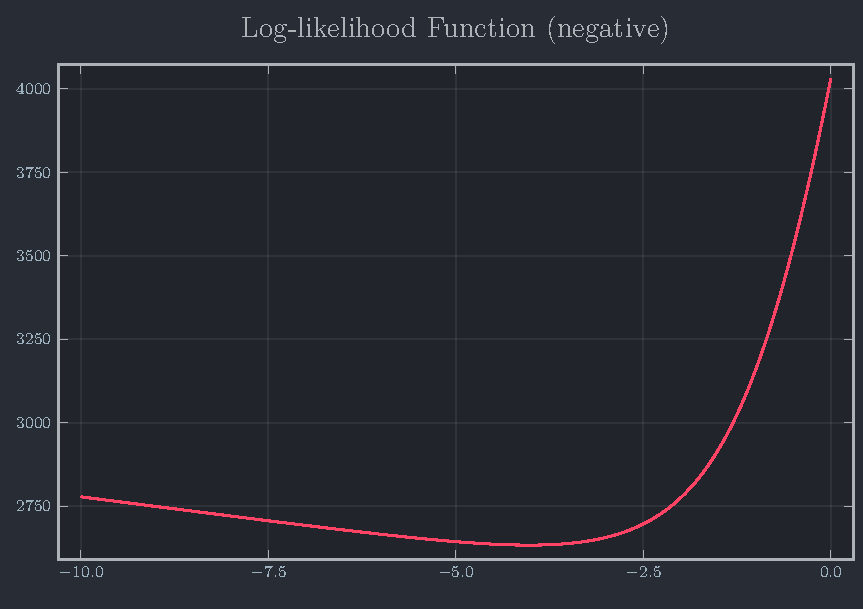
\includegraphics[width = \textwidth]{figures/Problem4.pdf}
\end{center}

\newpage
\section*{Appendix}
 	The first codefile named ``runfile.jl" runs the code.
 	%\jlinputlisting{runfile.jl}
	
 	The second codefile named ``functions.jl" contains the relevant functions.
 	%\jlinputlisting{functions.jl}
\end{document}